\documentclass[12pt,a4paper]{article}

\usepackage{epcc}
\usepackage{graphicx}
\usepackage{listings}
\usepackage{color}
\usepackage{amsmath}

\definecolor{mygreen}{rgb}{0,0.6,0}
\definecolor{mygray}{rgb}{0.5,0.5,0.5}
\definecolor{mymauve}{rgb}{0.58,0,0.82}

\lstset{
	backgroundcolor=\color{white},   % choose the background color; you must add \usepackage{color} or \usepackage{xcolor}; should come as last argument
	basicstyle=\footnotesize,        % the size of the fonts that are used for the code
	breakatwhitespace=false,         % sets if automatic breaks should only happen at whitespace
	breaklines=true,                 % sets automatic line breaking
	captionpos=b,                    % sets the caption-position to bottom
	commentstyle=\color{mygreen},    % comment style
	deletekeywords={...},            % if you want to delete keywords from the given language
	escapeinside={\%*}{*)},          % if you want to add LaTeX within your code
	extendedchars=true,              % lets you use non-ASCII characters; for 8-bits encodings only, does not work with UTF-8
	frame=single,	                   % adds a frame around the code
	keepspaces=true,                 % keeps spaces in text, useful for keeping indentation of code (possibly needs columns=flexible)
	keywordstyle=\color{blue},       % keyword style
	language=C,                 	 % the language of the code
	morekeywords={*,...},            % if you want to add more keywords to the set
	numbers=left,                    % where to put the line-numbers; possible values are (none, left, right)
	numbersep=5pt,                   % how far the line-numbers are from the code
	numberstyle=\tiny\color{mygray}, % the style that is used for the line-numbers
	rulecolor=\color{black},         % if not set, the frame-color may be changed on line-breaks within not-black text (e.g. comments (green here))
	showspaces=false,                % show spaces everywhere adding particular underscores; it overrides 'showstringspaces'
	showstringspaces=false,          % underline spaces within strings only
	showtabs=false,                  % show tabs within strings adding particular underscores
	stepnumber=5,                    % the step between two line-numbers. If it's 1, each line will be numbered
	stringstyle=\color{mymauve},     % string literal style
	tabsize=2,	                     % sets default tabsize to 2 spaces
	title=\lstname                   % show the filename of files included with \lstinputlisting; also try caption instead of title
}

\usepackage{hyperref}
\hypersetup{
	colorlinks=true, %set true if you want colored links
	linkcolor=black,  %choose some color if you want links to stand out
}

\newcommand{\sectionVspacing}{\vspace{15pt}}


\begin{document}

\title{Message Passing Programming Coursework Assignment}
\author{Exam number B136013}
\date{\today}

\makeEPCCtitle

\thispagestyle{empty}

\newpage
\clearpage

\tableofcontents

\newpage
\clearpage

\section{Introduction}
The project solves an image processing problem. It uses a two-dimensional domain decomposition in order to split the workload to the active processes. To achieve this we use MPI communication protocol for process communication. This approach arises a variety of challenges that need to be addressed, such as communication, decomposition, and boundary conditions.

\sectionVspacing

\section{Project Specification}
    There are a variety of project requirements in order to produce a correct output. On the one hand, there are fixed “sawtooth” boundary conditions in the horizontal direction. On the other hand, there are periodic boundary conditions in the vertical direction. This means that when a top process performs halo swap to fill the upper edge of the local table it receives it from the according to bottom process.

    Another specification is the terminate condition. The main loop of image reconstruction should finish when the maximum difference of a pixel in the image between the old and the value it's insignificant. This means that after some iterations when the produced image has not drastic variations from the previous the loop should be terminated.

\sectionVspacing

\section{Analysis}

    \subsection{MPP API}
    The implementation of the project uses mainly the basic functions of the MPI API. Some of these features perform non-blocking communication, create a virtual topology and use derived types.

        \paragraph{Communication}
            The corestone of the communication process are the MPI\_Isend and MPI\_Irecv functions. These methods are used for the halo swaps which are necessary for the calculations and the custom Scatter and Gather mechanisms. In the end of each of these procedures the program calls the MPI\_Wait function to ensure that there are not ongoing communications so the algorithm can resume its execution. In extension MPI\_Allreduce function has been used twice in the calculation procedure. First, to calculate the average pixel value which is part of the Output. Second, to calculate the max difference in the pixels between each iteration, and determine if the execution has to be stopped.

        \paragraph{Topology}
            In terms of the produced virtual topology, the main function was MPI\_Cart\_create that creates the new 2 dimension topology. Reorder of the given processes to the new topology is permited. In addition, methods like MPI\_Cart\_coords and MPI Cart rank are used identify the neighbor's ranks or coordinates.

        \paragraph{Derived Types}
            In order to reduce the code volume and avoid unnecessary memory allocations derived types are used extensively. Derived types such as row, column, and table are declared once in the main function. They can be found in the communication phase like the non-blocking functions. Their main goal is to avoid memory copies for the send and receive buffer. What we managed to is to read and write directly from the old buffer.

    \subsection{Design}
        The design and control flow of the project is basically the same as the case study with a different implementation. In the beginning, the program creates the virtual topology, does the decomposition of the problem and fill the necessary data structures for the rest of the execution. 

        In general, the algorithm has been designed to deal with any number of processes even for the occasion that they are not exactly divisible by the matrix size. The approach that we chose it that the border process was to calculate the extra workload. Different implementations for the derived types have been the tool to address this issue.

        Following the decomposition the master process reads the image and stores it to its master buffer. At the same time, all of the processes allocate the necessary buffers for the calculations.

        At this point the data exchange takes place. The master scatters the image which is stored in the master buffer directly to the edge buffers of the workers. When this part is done each process the old buffer filling it with white and fixes the horizontal borders if the worker has a part of the image which belongs to the left or right side.

        After the initialization is completed the main loop is ready to start. The calculation phase is decomposed as followed:
        \begin{enumerate}
          \item Halo swaps are sent to the neighbors if they exist, otherwise to MPI\_PROC\_NULL
          \item The middle calculations are computed (excluding those that require the halo swaps)
          \item The program waits to receive the halo swaps and then performs their part of calculations
          \item At specific intervals, the average pixel is logged and the program checks if the loop can be terminated
          \item If not the new buffer is overwritten to the old one
          \item Step 1 is executed
        \end{enumerate}

        In the end, the master gathers all of the old buffers and reconstructs the master buffer which will be written to the new output image.

    \subsection{Input/Output}
        The input of this experiment is an edge image and the number of process that are required to solve the problem. The output is a new reconstructed image based on the input. In addition, a print statement in the standard output that describes the input file, number of processes and running time in seconds. Last but not least, a Tab Seperated Value (TSV) file is generated that contains the average pixel's value between the fixed interval of the main calculation loop. The intervals have been defined to 100 loop iterations.

\sectionVspacing

\section{Evaluation}
    Evaluation has been done in order to find out if the program behaves as it should in terms of correctness and performance.

    \subsection{Tools and Building}
        For the development of this project the used programming language is C due to its performance in low-level calculations. The project is compiled using -O3 flag for serial optimization. In addition, GNU Make was selected for the build phase and Python to compare the output for testing reasons. To build the project just run: <make imagenew>

        Cirrus supercomputer is the platform that all of the experiments have been executed. In order to submit the job to the backend of Cirrus a Portable Batch System (PBS) has been developed. This file is a script to:
        \begin{enumerate}
          \item Build the project using GNU Make
          \item Load the Intel compilers
          \item Submit the MPI project to Cirrus with a variety of configurations.
        \end{enumerate}

        These configurations are:
        \begin{enumerate}
          \item A variety of process numbers from 1 to 32
          \item All of the edge images in resources/ folder
        \end{enumerate}

        To run it execute <qsub imagenew.pbs>.

        \paragraph{Noise}
            At this point we have to point out that each experiment has been executed multiple times. In our occasion, the image edgenew192x128.pgm running on 8 processes, has been executed 10 times then we calculate the mean running time and this value has been used to calculate the speedup for the specific configuration.

    \subsection{Correctness}
        First and foremost, before performance analysis, we have to ensure that the produced outputs are valid regardless of the number of processes that are used underneath. The approach is very simple. Once the job has been successfully executed, we run the serial program for all of the given input images and then store the outputs. The serial program has been modified to stop when there are no significant changes in the image's pixels between each step. To be more specific, the max different has been definied to be 0.1. It worths to mention that the termination condition has to remain the same in all of the executions because different conditions create different results. This comparison is made automatically through a Python script that uses the filecmp function. If the files are the same then our experiment is correct.


    \subsection{Performance}
        Performance analysis is essential for this experiment in order to compare our results and extract useful information of them. Speedup from the running time of our experiments. This a very useful measurement because we can decide how good our input scales for a variety of process. This would help us decide which is the optimal number of process to run if our budget or resources are limited.

        \subsubsection{Speedup}
            The timing of the experiment excludes Input and Output. The timing starts before the scatter and ends after the gather of the buffers. This decision has been made in order to take into consideration only the communication and calculation procedures.

            \paragraph{Small Input}
                Ideally as we increase the processors running the speedup should be increased accordingly but this is not the case for small problems. Let's take for example the case where the input image is 192x128 pixels. In Figure 1, it plain to see that the problem doen't scale as it should. When we use even more processors the speedup is slightly inclined. As a result, for the specific problem 4 or 5 process would be the best option. We don't have to waste 10 or 20 more of them if the speedup is not going to exceed 4.

                \begin{figure}[ht]
                    \centering
                    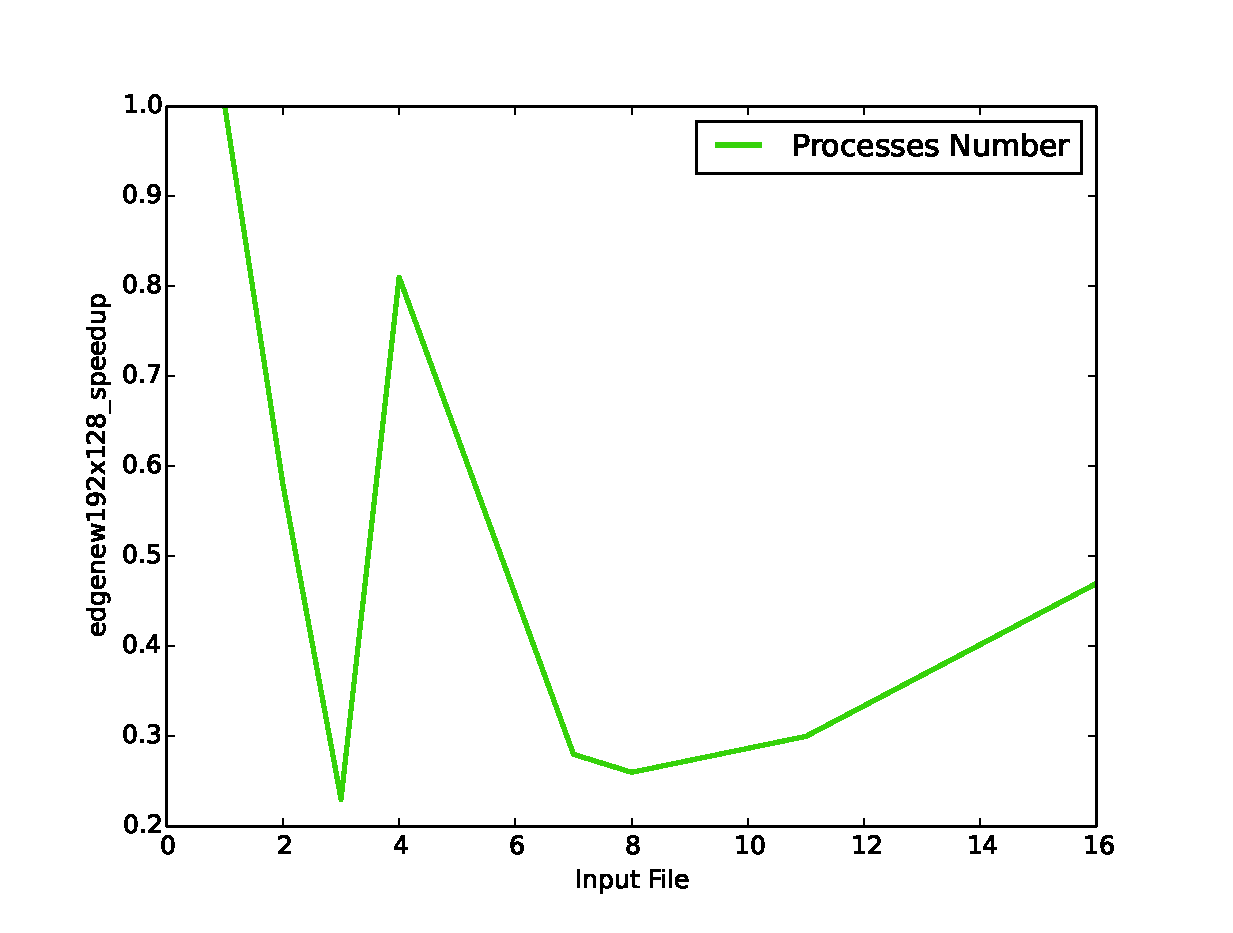
\includegraphics[scale=0.6]{../graphs/edgenew192x128_speedup.eps}
                    \caption{Speedup for image 192x128}
                    \label{speedup-192x128}
                \end{figure}
            
            \paragraph{Medium Input}
                As we increase the problem size 
                256x192 512x384
                \begin{figure}[ht]
                    \centering
                    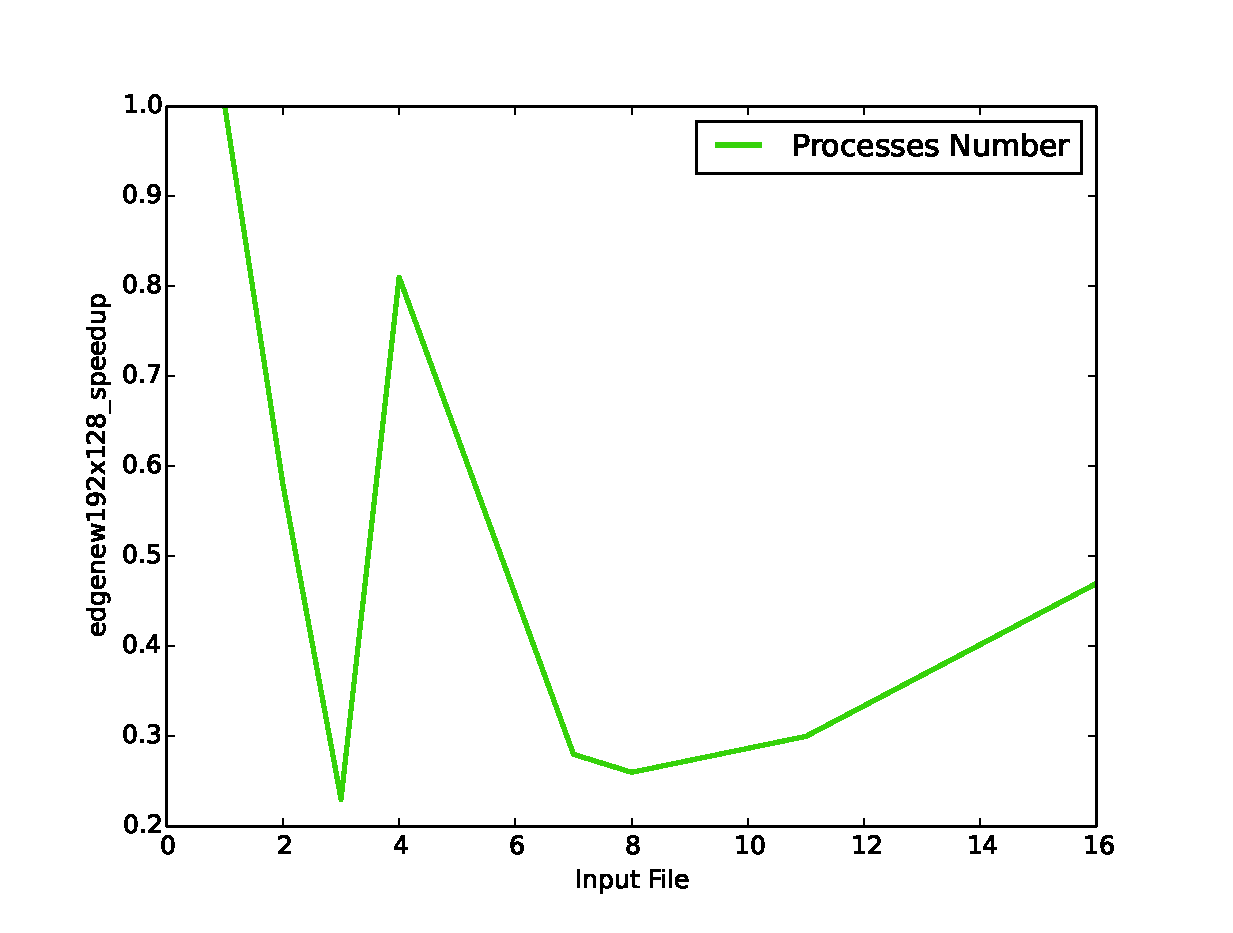
\includegraphics[scale=0.6]{../graphs/edgenew192x128_speedup.eps}
                    \caption{Speedup for image 192x128}
                    \label{speedup-192x128}
                \end{figure}

            \paragraph{Big Input}

            \paragraph{Enormous Input}




        \subsubsection{Average Pixel}
            Performance analysis for the average pixel results.
            % measure average time per iteration
            % are some inputs easier to be solved?
            % add tables???

\sectionVspacing

\section{Conclusion}
In conclusion.

\end{document}

% \begin{table}[h]
% 	\begin{center}
% 		\begin{tabular}{||l|c|l||}
% 			\hline
% 			{\bf Loop No} & {\bf Schedule}\\
% 			\hline
% 			Loop 1         &  schedule(guided, 4)\\
% 			Loop 2         &  schedule(dynamic, 16)\\
% 			\hline
% 		\end{tabular}
% 	\end{center}
% 	\caption{Best scheduler options on four (4) threads}
% 	\label{simple_table}
% \end{table}

% \lstinputlisting[language=C, firstline=2, lastline=3, caption=loops.c]{../template/loops_parallel-B136013.c}
